\documentclass[11pt]{article}
\usepackage[margin=3cm]{geometry}
\usepackage[utf8x]{inputenc}
\usepackage[english]{babel}
\usepackage[dvipsnames]{xcolor}
\usepackage{amsfonts}
\usepackage{amsmath}
\usepackage{amssymb}
\usepackage{url}
\usepackage{bookmark}
\usepackage{hyperref}
\usepackage{fancyhdr} 
\usepackage{youngtab}
\usepackage[
    type={CC},
    modifier={by-nc-sa},
    version={4.0},
]{doclicense}

% customized commands
\newcommand{\settag}[1]{\renewcommand{\theenumi}{#1}}
\newcommand{\R}{\mathbb{R}}
\newcommand{\real}{\mathbb{R}}
\newcommand{\complex}{\mathbb{C}}
\newcommand{\field}{\mathbb{F}}
\newcommand{\double}[1]{\mathbb{#1}} % Set to behave like that on word
\newcommand{\qed}{\hfill $\mathcal{Q}.\mathcal{E}.\mathcal{D}.\dagger$}
\newcommand{\tbf}[1]{\textbf{#1}}
\newcommand{\tit}[1]{\textit{#1}}
\newcommand{\contradiction}{$\longrightarrow\!\longleftarrow$}
\newcommand{\overbar}[1]{\mkern 1.5mu\overline{\mkern-1.5mu#1\mkern-1.5mu}\mkern 1.5mu}
\newcommand{\proof}{\tit{\underline{Proof:}}} % This equivalent to the \begin{proof}\end{proof} block
\newcommand{\proofforward}{\tit{\underline{Proof($\implies$):}}}
\newcommand{\proofback}{\tit{\underline{Proof($\impliedby$):}}}
\newcommand{\proofsuperset}{\tit{\underline{Proof($\supseteq$):}}}
\newcommand{\proofsubset}{\tit{\underline{Proof($\subseteq$):}}}
\newcommand{\trans}[3]{$#1:#2\rightarrow{}#3$}
\newcommand{\map}[3]{\text{$\left[#1\right]_{#2}^{#3}$}}
\newcommand{\dime}[1]{\text{dim}(#1)}
\newcommand{\mat}[2]{M_{#1 \times #2}(\R)}
\newcommand{\aug}{\fboxsep=-\fboxrule\!\!\!\fbox{\strut}\!\!\!}
\newcommand{\basecase}{\textsc{\underline{Basis Case:}} }
\newcommand{\inductive}{\textsc{\underline{Inductive Step:}} }
\newcommand{\norm}[1]{\left\lVert#1\right\rVert}
\newcommand{\independent}{\perp \!\!\! \perp}
% Call settag{\ldots} first to initialize, and then \para{} for a new paragraph
\newcommand{\va}{\mathbf{a}}
\newcommand{\vb}{\mathbf{b}}
\newcommand{\vv}{\mathbf{v}}
\newcommand{\vu}{\mathbf{u}}
\newcommand{\vw}{\mathbf{w}}
\newcommand{\vx}{\mathbf{x}}
\newcommand{\ve}{\mathbf{e}}
\newcommand{\vy}{\mathbf{y}}
\newcommand{\vz}{\mathbf{z}}
\newcommand{\vc}{\mathbf{c}}
\newcommand{\vm}{\mathbf{m}}
\newcommand{\vh}{\mathbf{h}}
\newcommand{\vzero}{\mathbf{0}}
% For convenience, I am setting both of these to refer to the same thing.
\newcommand{\ba}{\mathbf{a}}
\newcommand{\bb}{\mathbf{b}}
\newcommand{\bv}{\mathbf{v}}
\newcommand{\bu}{\mathbf{u}}
\newcommand{\bw}{\mathbf{w}}
\newcommand{\bx}{\mathbf{x}}
\newcommand{\be}{\mathbf{e}}
\newcommand{\by}{\mathbf{y}}
\newcommand{\bzero}{\mathbf{0}}
\newcommand{\boldf}{\mathbf{f}}
\newcommand{\bg}{\mathbf{g}}
\newcommand{\bm}{\mathbf{m}}

\title{\LARGE{Miscellaneous Notes on Regression}\\ \normalsize{Based on SJS and KNN}}
\author{\ccLogo \,\,Tingfeng Xia}
\date{Fall 2019, modified on \today}

\begin{document}
\maketitle
\section*{Preface}
Notes for STA302H1F fall offering, 2019 with Prof. Shivon Sue-Chee. These notes are based on the KNN and SJS text, in an aim for better understanding of the course material.
\doclicenseThis
\tableofcontents
\newpage

\section{Preliminaries}
\subsection{Distribution Theories}
\begin{itemize}
    \item Suppose $Y_1, Y_2 ,\dots, Y_n \overset{iid}{\sim} N(\mu, \sigma^2)$, and consider $s^{2}=\frac{1}{n-1} \sum_{i=1}^{n}\left(Y_{i}-\bar{Y}\right)^{2}$. Then,
        \begin{equation*}
            \frac{(n-1) s^{2}}{\sigma^{2}} \sim \chi^{2}_{(d f=n-1)}
        \end{equation*}
    \item Under the Normal Error SLR model, where $e_{i} \overset{iid}{\sim} N\left(0, \sigma^{2}\right)$, and $S^{2}=\frac{1}{n-2} \sum_{i=1}^{n} \hat{\mathrm{e}}_{i}^{2}=\frac{1}{n-2} \sum_{i=1}^{n}\left(Y_{i}-\hat{Y}_{i}\right)^{2}$ (Different from above!). Then,
        \begin{equation*}
            \frac{(n-2) S^{2}}{\sigma^{2}}=\frac{(n-2) S^{2} / S X X}{\sigma^{2} / S X X}=\sum_{i=1}^{n}\left(\frac{Y_{i}-\hat{Y}_{i}}{\sigma}\right)^{2} \sim \chi^{2}_{(d f=n-2)}
        \end{equation*}
    \item Let $Z\sim N(0,1)$, and $V\sim \chi^2_{(df=v)}$. Assume further that $Z\independent V$, then
        \begin{equation*}
            \frac{Z}{\sqrt{V / v}} \sim t_{(df=v)}
        \end{equation*}
    \item Under the Normal Error SLR model,
        \begin{equation*}
            \frac{\hat{\beta}_{1}-\beta_{1}}{\sqrt{\frac{S^{2}}{S X X}}} \sim t_{(n-2)}
        \end{equation*}
    \item Suppose $V \sim \chi_{(df=v)}^{2}$, $W \sim \chi_{(df=w)}^2$ and $V\independent W$. Then,
        \begin{equation*}
            \frac{V / v}{W / w} \sim F(v, w)
        \end{equation*}
    \item Suppose $Q\sim t_{(df=v)}$, then
        \begin{equation*}
            Q^2 \sim F(1,v)
        \end{equation*}
\end{itemize}

% TODO: CTD FROM
\section{Simple Linear Regression (Under Construction)}
\subsection{Ordinary Least Square}
\subsubsection{Simple Linear Regression Models}
The cost function to use in this case is the RSS, defined as
\begin{equation*}
    \mathrm{RSS}=\sum_{i=1}^{n} \hat{e}_{i}^{2}=\sum_{i=1}^{n}\left(y_{i}-\hat{y}_{i}\right)^{2}=\sum_{i=1}^{n}\left(y_{i}-b_{0}-b_{1} x_{i}\right)^{2}
\end{equation*}
We will now derive the OLS estimators as follows. 
\paragraph{Derivatives}
\begin{equation*}
    \frac{\partial \mathrm{RSS}}{\partial b_{0}}=-2 \sum_{i=1}^{n}\left(y_{i}-b_{0}-b_{1} x_{i}\right)=0
\end{equation*}
\begin{equation*}
    \frac{\partial \operatorname{RSS}}{\partial b_{1}}=-2 \sum_{i=1}^{n} x_{i}\left(y_{i}-b_{0}-b_{1} x_{i}\right)=0
\end{equation*}
\paragraph{Normal Equations} are obtained by rearranging
\begin{equation}
    \sum_{i=1}^{n} y_{i}=b_{0} n+b_{1} \sum_{i=1}^{n} x_{i}
\end{equation}
\begin{equation}
    \sum_{i=1}^{n} x_{i} y_{i}=b_{0} \sum_{i=1}^{n} x_{i}+b_{1} \sum_{i=1}^{n} x_{i}^{2}
\end{equation}
\paragraph{OLS Regressor}
\begin{equation*}
    \hat{\beta}_{0}=\bar{y}-\hat{\beta}_{1} \bar{x}
\end{equation*}
\begin{equation*}
    \hat{\beta}_{1}=\frac{\sum_{i=1}^{n} x_{i} y_{i}-n \overline{x y}}{\sum_{i=1}^{n} x_{i}^{2}-n \bar{x}^{2}}=\frac{\sum_{i=1}^{n}\left(x_{i}-\bar{x}\right)\left(y_{i}-\bar{y}\right)}{\sum_{i=1}^{n}\left(x_{i}-\bar{x}\right)^{2}}=\frac{S X Y}{S X X}
\end{equation*}
\paragraph{Estimating Variance of Residuals}
\begin{equation*}
    \hat{\sigma}^2 = S^{2}=\frac{\mathrm{RSS}}{n-2}=\frac{1}{n-2} \sum_{i=1}^{n} \hat{e}_{i}^{2} \quad \text{Unbiased Estimator}
\end{equation*}
\paragraph{Notes}
\begin{itemize}
    \item $\bar{\hat{e}}=0$, since $\sum \hat{e}_i = 0$ as the least square estimates minimizes RSS. (This is like a minimization goal where derivatives are taken w.r.t $\hat{e}_i$.)
    \item $S^2$ has $n-2$ degrees of freedom since we have estimated two parameters, namely $\beta_0$ and $\beta_1$.
\end{itemize}

\subsection{Inferences on Slope and Intercept}
\subsubsection{Inference Assumptions}
The following assumptions need to be made in order to preform inference
\begin{itemize}
    \item $Y$ is explained by $x$ through a simple linear regression model
        \begin{equation*}
            Y_{i}=\beta_{0}+\beta_{1} x_{i}+e_{i}(i=1, \ldots, n), \text { i.e., } \mathrm{E}\left(Y | X=x_{i}\right)=\beta_{0}+\beta_{1} x_{i}
        \end{equation*}
    \item Independent Errors, $e_i \independent e_j, \forall i \neq j$
    \item Homoscedasticity, $\text{Var}(e_i) = \sigma^2, \forall i$
    \item Normal Error: $e | X \sim N\left(0, \sigma^{2}\right)$
\end{itemize}
\subsubsection{Inference of Slope}
\paragraph{Distribution}
\begin{equation*}
    \hat{\beta}_{1} | X \sim N\left(\beta_{1}, \frac{\sigma^{2}}{S X X}\right)
\end{equation*}
\paragraph{Standardized Test Statistic (Var Known)}
\begin{equation*}
    Z=\frac{\hat{\beta}_{1}-\beta_{1}}{\sigma / \sqrt{S X X}} \sim N(0,1)
\end{equation*}
\paragraph{Test Statistic (Var Unknown)}
Recall that degress of freedom = sample size - number of mean parameters estimated. Then,
\begin{equation*}
    T=\frac{\hat{\beta}_{1}-\beta_{1}}{S / \sqrt{S X X}}=\frac{\hat{\beta}_{1}-\beta_{1}}{\operatorname{SE}\left(\hat{\beta}_{1}\right)} \sim t_{(df=n-2)} \quad \text{where}~~ S^2 = \frac{\sum_i \hat{e}_i^2}{n-2} 
\end{equation*}
\paragraph{Confidence Interval (Var Unknown)}
The $100(1- \alpha)\%$ CI is
\begin{equation*}
    CI \gets \hat{\beta}_1 \pm t^\ast_{()\alpha/2, df=n-2)} \times SE(\hat{\beta}_1) \equiv \hat{\beta}_1 \pm t^\ast_{(\alpha/2, df=n-2)} \frac{S}{\sqrt{S X X}}
\end{equation*}
\paragraph{Distribution Proof}
% TODO: add proof for distribution


\subsubsection{Inference of Intercept}
\paragraph{Distribution}
\begin{equation*}
    \hat{\beta}_{0} | X \sim N\left(\beta_{0}, \sigma^{2}\left(\frac{1}{n}+\frac{\bar{x}^{2}}{S X X}\right)\right)
\end{equation*}
\paragraph{Standardized Test Statistic (Var Known)}
\begin{equation*}
    Z=\frac{\hat{\beta}_{0}-\beta_{0}}{\sigma \sqrt{\frac{1}{n}+\frac{\bar{x}^{2}}{S X X}}} \sim N(0,1)
\end{equation*}
\paragraph{Test Statistic (Var Unknown)}
\begin{equation*}
    Z=\frac{\hat{\beta}_{0}-\beta_{0}}{S \sqrt{\frac{1}{n}+\frac{\bar{x}^{2}}{S X X}}} = \frac{\hat{\beta}_{0}-\beta_{0}}{\operatorname{SE}\left(\hat{\beta}_{0}\right)} \sim t_{(df=n-2)} \quad \text{where}~~ S^2 = \frac{\sum_i \hat{e}_i^2}{n-2} 
\end{equation*}
\paragraph{Confidence Interval (Var Unknown)}
\begin{equation*}
    CI \gets \hat{\beta}_0 \pm t^\ast_{()\alpha/2, df=n-2)} \times SE(\hat{\beta}_0) \equiv \hat{\beta}_0 \pm t^\ast_{(\alpha/2, df=n-2)} S\sqrt{\frac{1}{n}+\frac{\bar{x}^{2}}{S X X}}
\end{equation*}
\paragraph{Distribution Proof}
% TODO: add proof for distribution

\subsection{CI for \textit{Unknown} Population Regression Line}
Goal: Find a confidence interval for a unkown population regression line at $X = x^\ast$. The population regression line is given by
\begin{equation*}
    \mathrm{E}\left(Y | X=x^{*}\right)=\beta_{0}+\beta_{1} x^{*}
\end{equation*}
\paragraph{Distribution}
To get an estimate of the y value at $X = x^*$, we can use the regression output (evaluate the estimated regression line at $X = x^*$)
\begin{equation*}
    \hat{y}^{*}=\hat{\beta}_{0}+\hat{\beta}_{1} x^{*}
\end{equation*}
where we claim it follows the distribution
\begin{equation*}
    \hat{y}^{*}=\hat{y} | X=x^{*} \sim N\left(\beta_{0}+\beta_{1} x^{*}, \sigma^{2}\left(\frac{1}{n}+\frac{\left(x^{*}-\bar{x}\right)^{2}}{S X X}\right)\right)
\end{equation*}
\paragraph{Proof of Distribution}
The expectation follows directly from definition, and we will now show that the variance has the claimed value. Notice that $\text{Var}(\hat{\beta}_0|X) = \sigma^2 \left(\frac{1}{n} + \frac{\bar{x}^2}{SXX}\right)$, $\text{Var}(\hat{\beta}_1|X) = \frac{\sigma^2}{SXX}$ and $\text{Cov}(\hat{\beta}_0, \hat{\beta}_1 | X) = \frac{-\bar{x}\sigma^2}{SXX}$, then
\begin{align*}
    \text{Var}(\hat{y}|X = x^*)
    &= \text{Var}( \hat{\beta}_0 + \hat{\beta}_1 x^* |X = x^* ) \\
    &= \text{Var}(\hat{\beta}_0 | X = x^*) + \text{Var}(\hat{\beta}_1 x^* |X = x^*) + 2\text{Cov}(\hat{\beta}_1, \hat{\beta}_1 x^* | X = x^*) \\
    &= \sigma^2 \left(\frac{1}{n} + \frac{\bar{x}^2}{SXX}\right) + (x^*)^2 \frac{\sigma^2}{SXX} + 2x^* \left(\frac{-\bar{x}\sigma^2}{SXX}\right) \\
    &= \sigma^{2}\left(\frac{1}{n}+\frac{\left(x^{*}-\bar{x}\right)^{2}}{S X X}\right)
\end{align*}
\hfill \qed
\paragraph{Standardized Test Statistic (Var Known)}
\begin{equation*}
    Z=\frac{\hat{y}^{*}-\left(\beta_{0}+\beta_{1} x^{*}\right)}{\sigma \sqrt{\left(\frac{1}{n}+\frac{\left(x^{*}-\bar{x}\right)^{2}}{S X X}\right)}} \sim N(0,1)
\end{equation*}

\paragraph{Test Statistic (Var Knwon)}
\begin{equation*}
    T=\frac{\hat{y}^*-\left(\beta_{0}+\beta_{1} x^{*}\right)}{S \sqrt{\left(\frac{1}{n}+\frac{\left(x^{*}-\bar{x}\right)^{2}}{S X X}\right)}} \sim t_{(df=n-2)} \quad \text{where}~~S^2 = \frac{\sum_i \hat{e}_i^2}{n-2} 
\end{equation*}

\paragraph{Confidence Interval} A $100 (1 - \alpha) \%$ CI for $\mathrm{E}\left(Y | X=x^{*}\right)=\beta_{0}+\beta_{1} x^{*}$ is given by
\begin{align*}
    CI &\gets \hat{y}^{*} \pm t^\ast_{(\alpha / 2, df = n-2)} S \sqrt{\left(\frac{1}{n}+\frac{\left(x^{*}-\bar{x}\right)^{2}}{S X X}\right)} \\
    &\equiv \hat{\beta}_{0}+\hat{\beta}_{1} x^{*} \pm t^\ast_{(\alpha / 2, df =n-2)} S \sqrt{\left(\frac{1}{n}+\frac{\left(x^{*}-\bar{x}\right)^{2}}{S X X}\right)}
\end{align*}
\color{Thistle} 
Do note that this is only valid for $x^\ast$ values in the range of the original data values of $X$. Avoid extrapolation.
\color{Black}

\subsection{Prediction Intervals for Actual Value of Y}
\paragraph{Goal} Find a prediction interval for the actual value of Y at $x^*$, a given value of $X$.

\paragraph{Important Notes}
\begin{itemize}
    \item $E(Y | X = x^*)$, the expected value or average value of $Y$ for a given value $x^*$ of $X$, is what one would expect $Y$ to be in the long run when $X = x^*$. $E(Y | X = x^*)$ is therefore a fixed but unknown quantity whereas $Y$ can take a number of values when $X = x^*$.
    \item $E(Y | X = x^*)$, the value of the regression line at $X = x^*$, is entirely different from $Y^*$, a single value of $Y$ when $X = x^*$. In particular, $Y^*$ need not lie on the population regression line.
    \item A confidence interval is always reported for a parameter (e.g., $E(Y | X = x^*) = b_0 + b_1x^*$) and a prediction interval is reported for the value of a random variable (e.g., $Y^*$).
\end{itemize}

\paragraph{Difference Between CI and PI (My Thoughts)} The intrinsic difference is that: The CI we found above for $E(Y | X = x^*)$ is a CI for a fixed value. We are trying to find, in the long run where can we expect the regression line to lie given infinite samples. However, PI is trying to report for a specific value, possibly a not-already-observed new value, what is the range that it may appear in. PI captures more variablity. 

\paragraph{Distribution}
\begin{equation*}
    Y^{*}-\hat{y}^{*} \sim N\left(0, \sigma^{2}\left[1+\frac{1}{n}+\frac{\left(x^{*}-\bar{x}\right)^{2}}{S X X}\right]\right)
\end{equation*}

\paragraph{Test Statistic (Var Unknown)}
\begin{equation*}
    T=\frac{Y^*-\hat{y}^*}{S \sqrt{\left(1+\frac{1}{n}+\frac{\left(x^{*}-\bar{x}\right)^{2}}{S X X}\right)}} \sim t_{(df = n-2)}
\end{equation*}

\paragraph{Derivation of Distribution}
We base our prediction of $Y$ at $X = x^*$ (which is $Y^*$) on
\begin{equation*}
    \hat{y}^{*}=\hat{\beta}_{0}+\hat{\beta}_{1} x^{*}
\end{equation*}
The error (deviation, to be precise) of our prediction is 
\begin{equation*}
    Y^{*}-\hat{y}^{*}=\beta_{0}+\beta_{1} x^{*}+e^{*}-\hat{y}^{*}= \left(\mathrm{E}\left(Y | X=x^{*}\right)- \hat{y}^{*} \right) + e^{*}
\end{equation*}
that is, the deviation between $E(Y | X = x^*)$ and $y^*$ plus the random fluctuation $e^*$ (which represents the deviation of $Y^*$ from $E(Y|X = x^*)$). Thus the variability in the error for predicting a single value of $Y$ will exceed the variability for estimating the expected value of Y (because of the random error $e^*$). We have
\begin{equation*}
    \mathrm{E}\left(Y^{*}-\hat{y}^{*}\right)=\mathrm{E}\left(Y-\hat{y} | X=x^{*}\right)=0
\end{equation*}
and
\begin{equation*}
    \operatorname{Var}\left(Y^{*}-\hat{y}^{*}\right)=\operatorname{Var}\left(Y-\hat{y} | X=x^{*}\right)=\sigma^{2}\left[1+\frac{1}{n}+\frac{\left(x^{*}-\bar{x}\right)^{2}}{S X X}\right]
\end{equation*}









% FIXME: HERE!

\section{Diagnostics and Transformations for SLR}
\subsection{Valid and Invalid Data}
\subsubsection{Residuals}
One tool that we can use to validate a regression model is one or more plots of residuals (or standardized residuals). These plots will enable us to assess visually whether an appropriate model has been fit to the data no matter how many predictor variables are used. 

\paragraph{Expected Behavior} We expect that the residual graph to have no discernable pattern and centered at some value (0 in the case of standardized residual). Patterns such as curves, skewness et cetra indicates non-normal residuals. More on this in the below section.

\subsubsection{Reading Residual Plots}
\paragraph{Criterion} One way of checking whether a valid simple linear regression model has been fit is to plot residuals versus $x$ and look for patterns. If no pattern is found then this indicates that the model provides an adequate summary of the data, i.e., is a valid model. If a pattern is found then the shape of the pattern provides information on the function of $x$ that is missing from the model.  

\paragraph{Rationale} Suppose that the true model is a straight line (which we never know) defined as
\begin{equation}
    Y_{i}=\mathrm{E}\left(Y_{\mathrm{i}} | X_{i}=x_{i}\right)+e_{i}=\beta_{0}+\beta_{1} x_{i}+e_{i} \quad 
\end{equation}
where
\begin{equation*}
    e_i = \text{Random error on}~Y_i\quad \text{and} ~E(e_i) = 0
\end{equation*}
and we fit a regression line
\begin{equation*}
    \hat{y}_{i}=\hat{\beta}_{0}+\hat{\beta}_{1} x_{i}
\end{equation*}
Under the assumption that our regression line is very close to the true model, i.e. $\beta_0 \approx b_0$ and $\beta_1 \approx b_1$), we see
\begin{align*}
    \hat{e}_{i} 
    &= y_{i}-\hat{y}_{i} \\
    &= \beta_{0}+\beta_{1} x_{i} + e_i - \hat{\beta}_{0} - \hat{\beta}_{1} x_{i} \\
    &= \left(\beta_{0}-\hat{\beta}_{0}\right)+\left(\beta_{1}-\hat{\beta}_{1}\right) x_{i}+e_{i} \\
    &\approx e_i
\end{align*}
which means that our residuals resembles the random error! 

\subsection{Regression Diagnostics}
\paragraph{Catagorization}
\begin{itemize}
    \item \textbf{X-Direction Outlier, i.e. Leverage Point}: Away from the bulk of data in the $x$-direction. 
    \begin{itemize}
        \item \textbf{Good:} Not much chaneg after removing the data point, i.e. the data point originally was quite close to the regression line although away from the bulk of data in the $x$ direction. \textit{``A good leverage point is a leverage point which is NOT also an outlier.''}
        \item \textbf{Bad, Influential Point:} If its $Y$-value does not follow the pattern set by the other data points, i.e. a bad leverage point is a leverage point which is also an outlier. 
    \end{itemize}
    \item \textbf{Y-Direction Outlier} Trait: large residuals
\end{itemize}

\subsubsection{Leverage Point}
\paragraph{Defining The Hat}
The hat came from yet another representation of the $\hat{y}_i$. Recall that $\hat{y}_{i}=\hat{\beta}_{0}+\hat{\beta}_{1} x_{i}$, where $\hat{\beta}_{0}=\bar{y}-\hat{\beta}_{1} \bar{x}$, $\hat{\beta}_{1}=\sum_{j=1}^{n} c_{j} y_{j}$ and $c_{j}=\frac{x_{j}-\bar{x}}{S X X}$.
Then we have
\begin{align*}
    \hat{y}_{i}
    &=\bar{y}-\hat{\beta}_{1} \bar{x}+\hat{\beta}_{1} x_{i} 
    =\bar{y}+\hat{\beta}_{1}\left(x_{i}-\bar{x}\right) \\
    &=\frac{1}{n} \sum_{j=1}^{n} y_{j}+\sum_{j=1}^{n} \frac{\left(x_{j}-\bar{x}\right)}{S X X} y_{j}\left(x_{i}-\bar{x}\right) \\
    &=\sum_{j=1}^{n}\left[\frac{1}{n}+\frac{\left(x_{i}-\bar{x}\right)\left(x_{j}-\bar{x}\right)}{S X X}\right] y_{j} 
    =\sum_{j=1}^{n} h_{i j} y_{j}
\end{align*}
where we define
\begin{equation*}
    h_{i j}=\left[\frac{1}{n}+\frac{\left(x_{i}-\bar{x}\right)\left(x_{j}-\bar{x}\right)}{S X X}\right]
\end{equation*}
\paragraph{Property of The Hat}
Recall that $\sum_{j=1}^{n}\left[x_{j}-\bar{x}\right]=n\bar{x} - n\bar{x}=0$, then
\begin{equation*}
    \sum_{j=1}^{n} h_{i j}=\sum_{j=1}^{n}\left[\frac{1}{n}+\frac{\left(x_{i}-\bar{x}\right)\left(x_{j}-\bar{x}\right)}{S X X}\right]=\frac{n}{n}+\frac{\left(x_{i}-\bar{x}\right)}{S X X} \sum_{j=1}^{n}\left[x_{j}-\bar{x}\right]=1
\end{equation*}
Thus,
\begin{equation*}
    \hat{y}_{i}=h_{i i} y_{i}+\sum_{j \neq i} h_{i j} y_{j} \quad \text{where}~h_{i i}=\frac{1}{n}+\frac{\left(x_{i}-\bar{x}\right)^{2}}{\sum_{j=1}^{n}\left(x_{j}-\bar{x}\right)^{2}}
\end{equation*}
\paragraph{Defining Leverage} 
The term $h_{i i}=\frac{1}{n}+\frac{\left(x_{i}-\bar{x}\right)^{2}}{\sum_{j=1}^{n}\left(x_{j}-\bar{x}\right)^{2}}$ above is commonly known as the leverage of the $i$th data point. Notice the following in the definition of the leverage $h_{ii}$
\begin{itemize}
    \item The second term measures the proportion, in terms of squared deviation in $x$-direction over sum of square of total devaition in $x$-direction, of the $i$-th data point's deviation. When the second term tends to 1, meaning that $i$-th data point is some extreme outlier in the $x$-direction, then $h_{ii}$ would close to one, signifiying the `leverage'-ness. 
    \item Recall that $\sum_{j=1}^{n} h_{i j}=1$, then when $h_{i i} \cong 1$, $h_{ij}\rightarrow 0$ and
        \begin{equation*}
            \hat{y}_{i}=1 \times y_{i}+\text { other terms } \cong y_{i}
        \end{equation*}
    which means $\hat{y}_{i}$  will be very close to $y_i$, regardless of the rest dataset. 
    \item A point of high leverage (or a leverage point) can be found by looking at just the values of the $x$’s and not at the values of the $y$’s
\end{itemize}

\paragraph{Average of Leverage} For simple linear regression, 
\begin{equation*}
    \operatorname{average}\left(h_{i i}\right) = \frac{1}{n}\sum_{i = 1}^n h_{ii} =\frac{2}{n}
\end{equation*}

\paragraph{Identifying Leverage} Rule: $x_i$ is a high leverage (i.e., a leverage point) in a SLR model if 
\begin{equation*}
    h_{i i}>2 \times \operatorname{average}\left(h_{i i}\right)=2 \times 2 / n=4 / n
\end{equation*}

\paragraph{Dealing with `Bad' Leverage}
\begin{itemize}
    \item \textbf{Remove invalid data points;} Question the validity of the data points corresponding to bad leverage points, that is: Are these data points unusual or different in some way from the rest of the data? If so, consider removing these points and refitting the model without them. 
    \item \textbf{Fit a different regression model;} Question the validity of the regression model that has been fitted, that is: Has an incorrect model been fitted to the data? If so, consider trying a different model by including extra predictor variables (e.g., polynomial terms) or by transforming Y and/or x (which is considered later in this chapter).
\end{itemize}

\subsubsection{Standardized Residuals}
\paragraph{Problem of Non-constant Variance} Recall that 
\begin{equation*}
    h_{i j}=\frac{1}{n}+\frac{\left(x_{i}-\bar{x}\right)\left(x_{j}-\bar{x}\right)}{\sum_{j=1}^{n}\left(x_{j}-\bar{x}\right)^{2}}=\frac{1}{n}+\frac{\left(x_{i}-\bar{x}\right)\left(x_{j}-\bar{x}\right)}{S X X}
\end{equation*}
and (we will show this later)
\begin{equation*}
    \operatorname{Var}\left(\hat{e}_{i}\right)=\sigma^{2}\left[1-h_{i i}\right]
\end{equation*}
which is indeed non-constant for different data points. When  $h_{ii} \cong 1$ ($h_{ii}$ is very close to 1), the $i$-th data point is a leverage point and 
\begin{equation*}
    \operatorname{Var}(\hat{e}_i) = \sigma^{2}\left[1-h_{i i}\right] \approx 0 \quad \text{and} \quad \hat{y}_{i} \cong y_{i}
\end{equation*}
The above results intuitively makes sense: When $i$-th data point is a leverage, $\hat{e}_i$ will be small and it does not vary much (data point close to the estimated regression line). 

\paragraph{Derivation of Residual Variance (Not Important)}
Recall that
\begin{equation*}
    \hat{y}_{i}=h_{i i} y_{i}+\sum_{j \neq i} h_{i j} y_{j} \quad \text{where}~h_{i j}=\frac{1}{n}+\frac{\left(x_{i}-\bar{x}\right)\left(x_{j}-\bar{x}\right)}{\sum_{j=1}^{n}\left(x_{j}-\bar{x}\right)^{2}}=\frac{1}{n}+\frac{\left(x_{i}-\bar{x}\right)\left(x_{j}-\bar{x}\right)}{S X X}
\end{equation*}
Then,
\begin{equation*}
    \hat{e}_{i}=y_{i}-\hat{y}_{i}=y_{i}-h_{i i} y_{i}-\sum_{j \neq i} h_{i j} y_{j}=\left(1-h_{i i}\right) y_{i}-\sum_{j \neq i} h_{i j} y_{j}
\end{equation*}
Hence,
\begin{align*}
    \operatorname{Var}\left(\hat{e}_{i}\right) &= \operatorname{Var}\left(\left(1-h_{i i}\right) y_{i}-\sum_{j \neq i} h_{i j} y_{j}\right) \\
    &= \left(1-h_{i i}\right)^{2} \sigma^{2}+\sum_{j \neq i} h_{i j}^{2} \sigma^{2} \\
    &= \sigma^{2}\left[1-2 h_{i i}+h_{i i}^{2}+\sum_{j \neq i} h_{i j}^{2}\right] \\
    &=\sigma^{2}\left[1-2 h_{i i}+\sum_{j} h_{i j}^{2}\right]
\end{align*}
Notice that 
\begin{align*} 
    \sum_{j=1}^{n} h_{i j}^{2} &=\sum_{j=1}^{n}\left[\frac{1}{n}+\frac{\left(x_{i}-\bar{x}\right)\left(x_{j}-\bar{x}\right)}{S X X}\right]^{2} \\ &=\frac{1}{n}+2 \sum_{j=1}^{n} \frac{1}{n} \times \frac{\left(x_{i}-\bar{x}\right)\left(x_{j}-\bar{x}\right)}{S X X}+\sum_{j=1}^{n} \frac{\left(x_{i}-\bar{x}\right)^{2}\left(x_{j}-\bar{x}\right)^{2}}{S X X^{2}} \\ &=\frac{1}{n}+0+\frac{\left(x_{i}-\bar{x}\right)^{2}}{S X X} \\ &=h_{i i} 
\end{align*}
So,
\begin{equation*}
    \operatorname{Var}\left(\hat{e}_{i}\right)=\sigma^{2}\left[1-2 h_{i i}+h_{i i}\right]=\sigma^{2}\left[1-h_{i i}\right]
\end{equation*}
and
\begin{equation*}
    \color{Thistle}{\operatorname{Var}\left(\hat{y}_{i}\right)} \color{Black}=\operatorname{Var}\left(\sum_{j=1}^{n} h_{i j} y_{j}\right)=\sum_{j \neq i} h_{i j}^{2} \operatorname{Var}\left(y_{j}\right)=\sigma^{2} \sum_{j} h_{i j}^{2}=\color{Thistle}{\sigma^{2} h_{i i}}
\end{equation*}

\paragraph{Overcome with Standardization} The above problem of each $\hat{e}_i$ having different variances could be overcame by standardizing the residuals. The $i$-th standardized residual is defined as (notice that the $s = \hat{\sigma}$ is the estimated variance in the SLR settings)
\begin{equation*}
    r_{i}=\frac{\hat{e}_{i}}{s \sqrt{1-h_{i i}}}\quad \text{where}~ s=\sqrt{\frac{1}{n-2} \sum_{j=1}^{n} \hat{e}_{j}^{2}}
\end{equation*}

\paragraph{Advantages of Standardization} 
\begin{itemize}
    \item When points of high leverage exist, instead of looking at residual plots, it is generally more informative to look at plots of standardized residuals since plots of the residuals will have nonconstant variance even if the errors have constant variance.
    \item When points of high leverage do not exist, there is gener- ally little difference in the patterns seen in plots of residuals when compared with those in plots of standardized residuals.
    \item The other advantage of standardized residuals is that they immediately tell us how many estimated stand- ard deviations any point is away from the fitted regression model. 
\end{itemize}

\paragraph{Recognizing Outliers Using Standardized Residuals} 
\begin{itemize}
    \item An \textbf{outlier} is a point whose standardized residual falls outside the interval from -2 to 2, i.e. $|r_i| > 2$
    \item A \textbf{Bad Leverage Point} is a leverage point whose standardized residual falls outside the interval from -2 to 2, i.e. $|r_i| > 2 \wedge h_{ii} > \frac{4}{n}$
    \item A \textbf{Good Leverage Point} is a leverage point whose standardized residual falls inside the interval from -2 to 2, i.e. $|r_i| \leq 2 \wedge h_{ii} > \frac{4}{n}$
    \item \textbf{Dealing with large datasets:} In this case, we should change the above criterion to $r_i| > 4$ and $r_i| \leq 4$ respectively. This is to give allowance for more occurence of rare events in a large data set.
\end{itemize}

\paragraph{Correlation Between Residuals} Even if the errors are independent (homogeneous), i.e. $e_i \independent e_j~(i \neq j)$, the residuals are still correlated. It can be shown that the covariance and the correlation is given by
\begin{equation*}
    \operatorname{Cov}\left(\hat{e}_{i}, \hat{e}_{j}\right)=-h_{i j} \sigma^{2}(i \neq j)
\end{equation*}
\begin{equation*}
    \operatorname{Corr}\left(\hat{e}_{i}, \hat{e}_{j}\right)=\frac{-h_{i j}}{\sqrt{\left(1-h_{i i}\right)\left(1-h_{i j}\right)}}(i \neq j)
\end{equation*}
Such correlation could be safely ignored in practice. They are usualy given raise by inherent correlation such as data collected over time.

\subsubsection{Recommendations for Handling Outliers \& Leverage}
We have discussed multiple ways of assessing outliers and talked about the way to deal with them by removing them. However, it is not always a good idea to delete them for the following reasons:
\begin{itemize}
    \item Points should not be routinely deleted from an analysis just because they do not fit the model. Outliers and bad leverage points are signals, flagging potential problems with the model.
    \item Outliers often point out an important feature of the problem not considered before. They may point to an alternative model in which the points are not an outlier. In this case it is then worth considering fitting an alternative model. 
\end{itemize}

\subsubsection{Influence of Certain Cases}
It can sometimes be the case that certain data points in a data set are drastically controlling the entire regression model (the model has payed too much attention to them). We now develop methods where we measure the ``importance'' of a data point.

\paragraph{Cook's Distance} First, define (recall if already defined) the following notation
\begin{itemize}
    \item $\hat{{y}}_{j(i)}$ means the the fitted value of the $j$-th data point on the regression line obtained by removing the $i$-th case. 
    \item $S^2 = \frac{1}{n-2} \sum_{j=1}^n \hat{e}_j^2$ is the variance (Original MSE) of the \color{Thistle}{total regression model}. \color{black}
    \item $r_{i}=\frac{\hat{e}_{i}}{s \sqrt{1-h_{i i}}}\quad \text{where}~ s=\sqrt{\frac{1}{n-2} \sum_{j=1}^{n} \hat{e}_{j}^{2}}$
\end{itemize}
Then, the Cook's Distance of the $i$-th datapoint is given by
\begin{equation*}
    \color{OliveGreen}
    D_{i}=\frac{\sum_{j=1}^{n}\left(\hat{y}_{j(i)}-\hat{y}_{j}\right)^{2}}{2 S^{2}} = \frac{r_{i}^{2}}{2} \frac{h_{i i}}{1-h_{i i}}
\end{equation*}
where we should note that $D_i$ may be large due to large $r_i$, or large $h_{ii}$ or both.

\paragraph{Rule: Cook's Distance} 
\begin{itemize}
    \item A point is noteworthy if
        \begin{equation*}
            D_i > \frac{4}{n-2}
        \end{equation*}
    \item In practice, look for gaps in the values of Cook's Distance and not just whether one value exceeds tyhe suggested cut off.
\end{itemize}

\subsubsection{Normality of the Errors}
The assumption of normal errors is (especially) needed in small samples for the validity of $t$-dist based tests and inferences. This assumption is generally checked by looking at the distribution of the residuals or standardized residuals. Recall that the $i$-th least squares residuals is given by $\hat{e}_{i}=y_{i}-\hat{y}_{i}$. We will now show $\hat{e}_{i}=e_{i}-\sum_{j=1}^{n} h_{i j} e_{j}$. First, in the derivation we will need these two facts
\begin{equation*}
    \sum_{i=1}^{n} h_{i j}=1
\end{equation*}
and 
\begin{equation*}
    \sum_{j=1}^{n} x_{j} h_{i j}=\sum_{j=1}^{n}\left[\frac{x_{j}}{n}+\frac{\left(x_{i}-\bar{x}\right)\left(x_{j}-\bar{x}\right) x_{j}}{S X X}\right]=\bar{x}+\frac{\left(x_{i}-\bar{x}\right) S X X}{S X X}=x_{i}
\end{equation*}
We then proceed as follows
\begin{align*} 
    \hat{e}_{i} &=y_{i}-\hat{y}_{i} =y_{i}-h_{i i} y_{i}-\sum_{j \neq i} h_{i j} y_{j} \\ 
    &=y_{i}-\sum_{j=1}^{n} h_{i j} y_{j} \\ 
    &=\beta_{0}+\beta_{1} x_{i}+e_{i}-\sum_{j=1}^{n} h_{i j}\left(\beta_{0}+\beta_{1} x_{j}+e_{j}\right) \\ 
    &=\beta_{0}+\beta_{1} x_{i}+e_{i}-\beta_{0}-\beta_{1} x_{i}-\sum_{j=1}^{n} h_{i j} e_{j} \\ 
    &\color{Thistle}{=e_{i}-\sum_{j=1}^{n} h_{i j} e_{j}}
\end{align*}
\hfill \qed \newline
The above result showed that the $i$-th least squares residual is equal to $e_i$ minus a weighted sum of all the $e$'s. There are two cases to consider,
\begin{itemize}
    \item In small to moderate samples, the second term could dominate the first and first and the residuals can look like they come from a normal distribution even if the errors do not. 
    \item When $n$ is large, the second term in the derived result (thistle colored) has a much smaller variance than that of the first term and as such the first term dominates the last equation. 
\end{itemize}
\textbf{Conclusion:} For large samples, the residuals can be used to assess normality of the errors.

\paragraph{Assessment Using Normal Q-Q}
A normal probability plot of the standardized residuals is obtained by plotting the ordered standardized residuals on the vertical axis against the expected order statistics from a standard normal distribution on the horizontal axes. If the resulting plot produces points ``close'' to a straight line then the data are said to be consistent with that from a normal distribution. On the other hand, departures from linearity provide evidence of non-normality. 
\begin{center}
    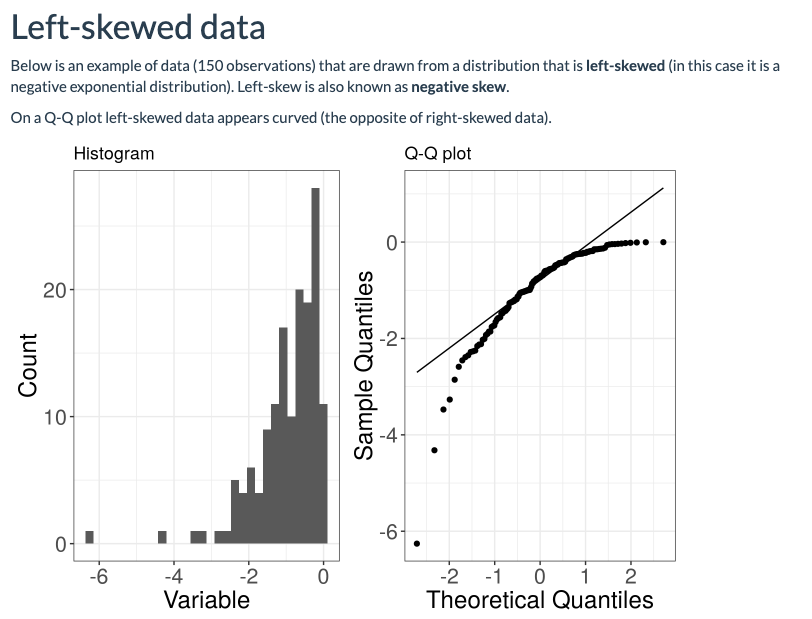
\includegraphics[scale=0.27]{img/qq_left.png}
    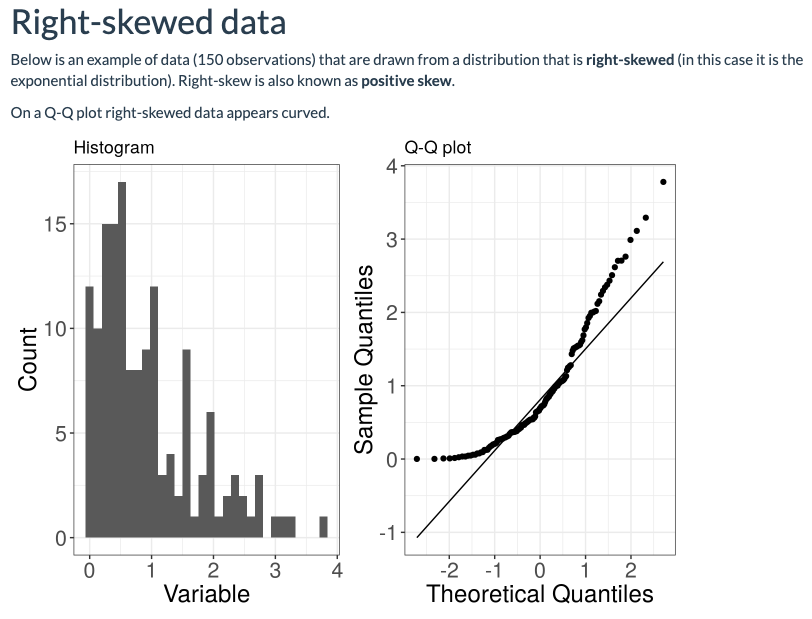
\includegraphics[scale=0.27]{img/qq_right.png}
    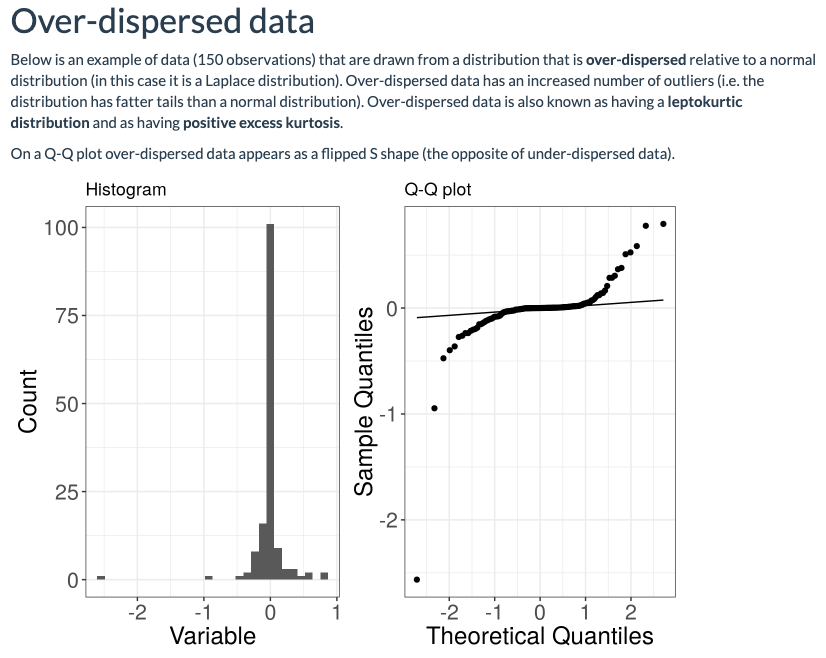
\includegraphics[scale=0.26]{img/qq_over.png}
    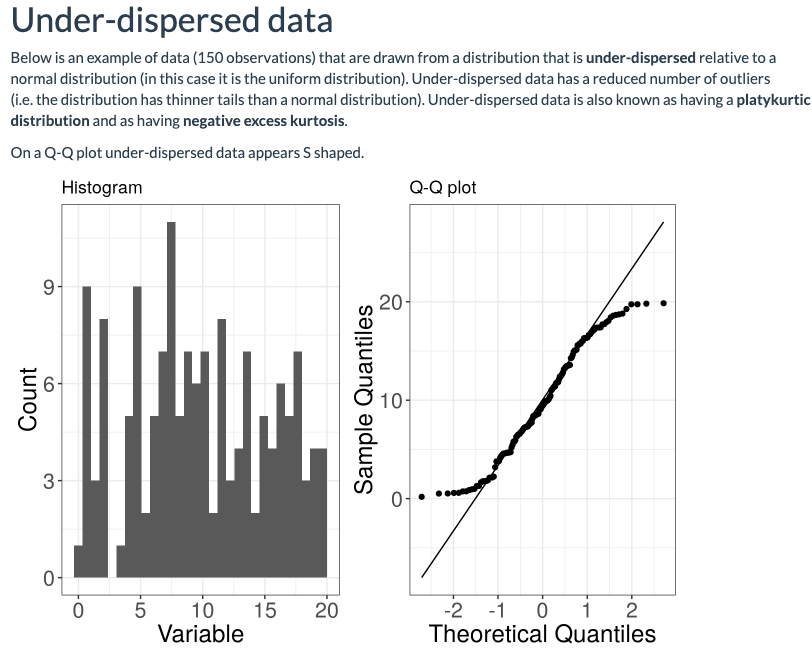
\includegraphics[scale=0.26]{img/qq_under.png}
\end{center}
The above four are figures that I borrowed from \url{http://www.ucd.ie/ecomodel/Resources/QQplots_WebVersion.html} which illustrates how to interpret QQ plots with non-normal behavior.

\subsubsection{Constant Variance (Homoscedasticity)}
A crucial assumption in any regression analusis is that errors have constant variance. \color{BurntOrange} Notice the difference between error and residual, we have demonstrated in \textbf{(3.2.2 Standardized Residuals)} that residuals are not of constant variance. \color{Black} There are two general methods that we can adopt to overcome this issue, namely (noth of which will be discussed later)
\begin{itemize}
    \item Transformations
    \item Weighted Least Squares
\end{itemize}
\color{Red}
\textit{\textbf{Important:} Ignoring nonconstant variance when it exists invalidates all inferential tools, including p-values, CI, PI, et cetra!}
\color{Black}

\paragraph{Behavior of Non-Homoscedasticity} For example, on the plot explanatory var against standardized residuals, we might see that as $x$ increases, the residuals are more spread out, indicating an increasing trend in the variance. 

\paragraph{Checking for Constant Variance} To check this, check the plot of
\begin{equation*}
    |\text{ Residuals }|^{0.5} \text { against } x \quad \text{or} \quad |\text { Standardized Residuals }|^{0.5} \text { against } x
\end{equation*}
The power of $0.5$ here is used to reduce skewness in the absolute values. In the above mentioned example where the residuals become more spread out as $x$ increases, the plot $|\text { Standardized Residuals }|^{0.5} \text { against } x$ will have an overall increasing trend! \color{BurntOrange} This is essentially mirroring all the points to the positive side (and de-skew) to observe a general trend. \color{Black}

\subsection{Transformation}
\subsubsection{Variance Stablizing Transformations}
\paragraph{Goal} When non-constant cariance exists, it is often possible to transform one or both of the regression variables to preduce a model in which the error variance is constant. 

\paragraph{Delta Method, Poisson} Suppose that $Y\sim \operatorname{Poi}(\mu = \lambda)$ and we want to find the appropriate transformation of $Y$ for stablizing variance. \color{Thistle}{In this case, square root is the appropriate transformation to apply.} \color{Black} We will now justify this choice. Consider the McLauren Series expension
\begin{equation*}
    f(Y)=f(\mathrm{E}(Y))+f^{\prime}(\mathrm{E}(Y))(Y-\mathrm{E}(Y))+\ldots
\end{equation*}
According to the delte rule, the first order variance term is obtained by taking variance on both sides of the above equation, which yields
\begin{equation*}
    \operatorname{Var}(f(Y)) \simeq\left[f^{\prime}(\mathrm{E}(Y))\right]^{2} \operatorname{Var}(Y)
\end{equation*}
Using the proposed transformation $f(Y)=Y^{0.5}$ and recall from properties of Poisson Random Variable that $\operatorname{Var}(Y)=\lambda=\mathrm{E}(Y)$, then
\begin{equation*}
    \operatorname{Var}\left(Y^{0.5}\right) \simeq\left[0.5(\mathrm{E}(Y))^{-0.5}\right]^{2} \operatorname{Var}(Y)=\left[0.5 \lambda^{-0.5}\right]^{2} \lambda=\mathrm{constant}
\end{equation*}
\color{Thistle} \textbf{Rule of Thumb:} When both $Y$ and $X$ are measured in the same units then it is often natural to consider the same transformation for both $X$ and $Y$ \color{Black} \newline \newline
Hence in this case our regression model would be
\begin{equation*}
    Y=\beta_{0}+\beta_{1} x+e
\end{equation*}
where
\begin{equation*}
    Y \gets \sqrt{Y} \quad \text{and} \quad x \gets \sqrt{x}
\end{equation*}

\subsubsection{Logarithms to Estimate Percentage Effects}
Consider the regression model
\begin{equation*}
    \log (Y)=\beta_{0}+\beta_{1} \log (x)+e
\end{equation*}
The slope,\footnote{Notice that the first step is possible since here we are considering the regression straight line}
\begin{align*}
    \beta_{1} &=\frac{\Delta \log (Y)}{\Delta \log (x)} =\frac{\log \left(Y_{2}\right)-\log \left(Y_{1}\right)}{\log \left(x_{2}\right)-\log \left(x_{1}\right)}
    =\frac{\log \left(Y_{2} / Y_{1}\right)}{\log \left(x_{2} / x_{1}\right)} \\
    &\cong \frac{Y_{2} / Y_{1}-1}{x_{2} / x_{1}-1}\left(\text { using } \log (1+z) \cong z \text { and assuming } \beta_{1} \text { is small }\right) \\
    &=\frac{100\left(Y_{2} / Y_{1}-1\right)}{100\left(x_{2} / x_{1}-1\right)} =\frac{\% \Delta Y}{\% \Delta x}
\end{align*}

\paragraph{Interpretation} We showed above that $\% \Delta Y \simeq \beta_{1} \times \% \Delta x$. Thus for every \(1 \%\) increase in \(x,\) the model predicts a \(\beta_{1} \%\) increase in \(Y\) (provided
\(\beta_{1}\) is small).


\section{Weighted Least Square Regression}
\subsection{Motivation and Set-Up}
Consider the straight line (simple) linear regression model
\begin{equation*}
    Y_{i}=\beta_{0}+\beta_{1} x_{i}+e_{i} \quad \text{where}~~ e_i \sim N \left(0, \frac{\sigma^2}{w_i}\right)
\end{equation*}
For the weight $w_i$, we should note the following
\begin{itemize}
    \item $w_i \rightarrow \infty \implies Var(e_i) \rightarrow 0$. In this case, the estimates of the regression parameters $\beta_0, \beta_1$ should be such that the fitted line at $x_i$ should be very close to $y_i$. (Small variance means more strict in terms of deviation from the regressin line, corresponding to a larger emphasis on the $i$-th data point.)
    \item If $w_i$ is some small value, then the variance of the $i$-th data point would be quite large. In this case, we have a loose restriction of the deviation of the $i$-th data point from the regression line meaning that litte emphasis is taken for this data point.
    \item $w_i \rightarrow 0 \implies Var(e_i) \rightarrow \infty$. In this case, we have the variance tending to infinity. Meaning that there is absolutely no restriction/emphasis on the $i$-th data point and it could be simply removed from the set.
\end{itemize}
We define the cost function, WRSS as
\begin{equation*}
    \mathrm{WRSS}=\sum_{i=1}^{n} w_{i}\left(y_{i}-\hat{y}_{W_i}\right)^{2}=\sum_{i=1}^{n} w_{i}\left(y_{i}-b_{0}-b_{1} x_{i}\right)^{2}
\end{equation*}
and the estimators $\bb = [b_0, b_1]^T$ are derived using MLE. 

\paragraph{Intuition behind WRSS} This cost function may seem wierd at first glance, but it intuitively makes sense. Notice that when $w_i$ is large, the $i$-th lost term $w_{i}\left(y_{i}-\hat{y}_{W_i}\right)^{2}$ is payed more emphasis on. On the contrary, when $w_0 \rightarrow 0$, the term $\rightarrow 0$. (Indeed, when Variance of the term $\rightarrow \infty$ we just neglect it.)

\subsection{Deriving ML Estimators}
\paragraph{Derivatives}
\begin{equation}
    \frac{\partial \mathrm{WRSS}}{\partial b_{0}}=-2 \sum_{i=1}^{n} w_{i}\left(y_{i}-b_{0}-b_{1} x_{i}\right)=0
\end{equation}
\begin{equation}
    \frac{\partial \mathrm{WRSS}}{\partial b_{1}}=-2 \sum_{i=1}^{n} w_{i} x_{i}\left(y_{i}-b_{0}-b_{1} x_{i}\right)=0
\end{equation}
\paragraph{Normal Equations} Obtained from rearranging the above equations, we will call them Normal Eq1 and Normal Eq2 respectively for later reference.
\begin{equation}
    \sum_{i=1}^{n} w_{i} y_{i}=b_{0} \sum_{i=1}^{n} w_{i}+b_{1} \sum_{i=1}^{n} w_{i} x_{i}
\end{equation}
\begin{equation}
    \sum_{i=1}^{n} w_{i} x_{i} y_{i}=b_{0} \sum_{i=1}^{n} w_{i} x_{i}+b_{1} \sum_{i=1}^{n} w_{i} x_{i}^{2}
\end{equation}
\paragraph{Rearranging} Use $\text{Normal Eq1} \times\sum_{i=1}^{n} w_{i} x_{i}$ and $\text{Normal Eq2}\times\sum_{i=1}^{n} w_{i}$
\begin{equation}
    \sum_{i=1}^{n} w_{i} x_{i} \sum_{i=1}^{n} w_{i} y_{i}=b_{0} \sum_{i=1}^{n} w_{i} \sum_{i=1}^{n} w_{i} x_{i}+b_{1}\left(\sum_{i=1}^{n} w_{i} x_{i}\right)^{2}
\end{equation}
\begin{equation}
    \sum_{i=1}^{n} w_{i} \sum_{i=1}^{n} w_{i} x_{i} y_{i}=b_{0} \sum_{i=1}^{n} w_{i} \sum_{i=1}^{n} w_{i} x_{i}+b_{1} \sum_{i=1}^{n} w_{i} \sum_{i=1}^{n} w_{i} x_{i}^{2}
\end{equation}
\paragraph{WLS Slope Estimator} \footnote{Note that $\bar{x}_{W}=\sum_{i=1}^{n} w_{i} x_{i} / \sum_{i=1}^{n} w_{i}$ and $\bar{y}_{W}=\sum_{i=1}^{n} w_{i} y_{i} / \sum_{i=1}^{n} w_{i}$}
\begin{align}
    \hat{\beta}_{1W} &= \frac{\sum_{i=1}^{n} w_{i} \sum_{i=1}^{n} w_{i} x_{i} y_{i}-\sum_{i=1}^{n} w_{i} x_{i} \sum_{i=1}^{n} w_{i} y_{i}}{\sum_{i=1}^{n} \sum_{i=1}^{n} w_{i} x_{i}^{2}-\left(\sum_{i=1}^{n} w_{i} x_{i}\right)^{2}} \\
    &= \frac{\sum_{i=11}^{n} x_{i}\left(x_{i}-\bar{x}_{W}\right)\left(y_{i}-\bar{y}_{W}\right)}{\sum_{i=1}^{n} w_{i}\left(x_{i}-\bar{x}_{W}\right)^{2}}
\end{align}
\paragraph{WLS Intercept Estimator}
\begin{equation}
    \hat{\beta}_{0 W}=\frac{\sum_{i=1}^{n} w_{i} y_{i}}{\sum_{i=1}^{n} w_{i}}-\hat{\beta}_{1 W} \frac{\sum_{i=1}^{n} w_{i} x_{i}}{\sum_{i=1}^{n} w_{i}} = \bar{y}_{w}-\hat{\beta}_{1 W} \bar{x}_{W}
\end{equation}

\section{Multiple Linear Regression (Under Construction)}




\end{document}
